\section{Stimuli Design} \label{sec:Stim}

The following section will describe different standards of designing experiments, where the impact of a given stimuli is used to assess the subsequent brain activation. The impact of stimuli on the hemodynamic response and how it is transformed into the hemodynamic response function (HRF) used analysis will be further explained. \\
In order to accomplish a well designed experiment, the researcher must consider the multiple types of stimuli delivered, including the form and duration of these. The researcher must be aware of the timing of events in the scanning session and any responses provoked. Additionally, the researcher should have general knowledge of where in the brain activation is seen and how the hemodynamic response will be presented. \cite{Moayedi2018} \\
Doing cognitive experiments using fMRI, two main design types are utilized, by either using a block- or event-related design. Event-related design is inducing a series of very short lasting stimuli used to investigate single hemodynamic response. A characteristic of this method is that it permits the possibility of increasing and decreasing the interval between stimuli. Thereby the theoretical likelihood of subject confounds should be reduced as the interval would not become predictable. Event-related stimuli design further allows more temporals characteristics to be inspected, compared to a block design. Characteristics could be hemodynamic response in duration and amplitude. \cite{Chee2003}  \\
Block design works by performing a series of less but longer stimuli. Block designs are ideal for experiments involving detection of small differences in BOLD signal across various test conditions where its statistical power is superior. Furthermore, if there is artifacts present they are more easily detected in the signal time course, because of the signals temporal structure. A block design is easier to design than an event-related, as randomization of intervals of stimuli is not required. The design instead focuses on the total number of stimuli used, block length, inter stimulus interval, block length and TR. An illustration of both design types can be found in \figref{fig:back:e_vs_b}. \cite{Chee2003}  \\     
To enable use of the hemodynamic response in fMRI analysis, it needs to be transformed in order to represent the ideal physiologic response to the stimulus. Thus, portraying the biological delay from stimuli to response. Therefore stimulus in the design is combined with the hemodynamic response function through convolution. Thus making a function that models how the BOLD signal would be represented if the voxel activity increased in a given area each time stimuli is induced. \cite{Moayedi2018}

\begin{figure}[H]                 
	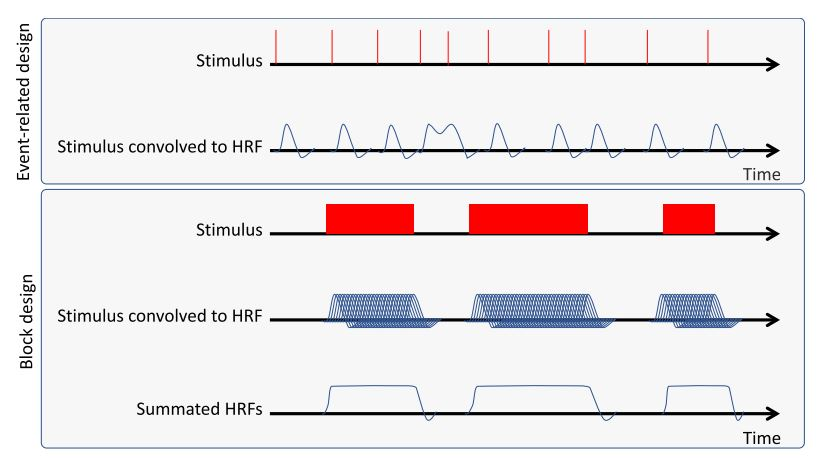
\includegraphics[width=.8\textwidth]{figures/aBackground/event_vs_block}  
	\caption{The top image show the event-related stimuli design and the stimulus convolved with the hemodynamic response function. The lower image depicts a block design, the stimulus convolved with hemodynamic response function and the summated HRF response.  \cite{Moayedi2018}}
	\label{fig:back:e_vs_b} 
\end{figure}

 

